\section{Calibration Framework}
\label{sec:method}

\subsection{From Scores to Thresholds}
A score alone does not trigger maintenance; a threshold does. We compare four thresholding mechanisms on identical scores. All mechanisms estimate or maintain a quantile of the score distribution and alarm when $\st>\qt$. Only the static rule uses no target information beyond what is deployed at time zero.

\subsection{Static Source Calibration}
Given source-calibrated scores (a held-out 20\% of source-normal windows), the split-conformal threshold is the empirical $(1-\alphaNom)$ quantile $\qsrc$. This is the standard practice implied by \cite{lei2018} and is optimal under exchangeability between calibration and deployment windows---precisely what cross-domain shift breaks.

\subsection{Online Adaptive Conformal Inference (ACI)}
We maintain $\qt$ with the \emph{relative-gain} (scale-free) form of adaptive conformal inference \cite{aci2021}
\begin{equation}
q_{t+1} = q_t + \gamma \cdot \max(|q_t|,\epsilon)\, \bigl(\mathbb{1}[\st > q_t] - \alphaNom\bigr),
\label{eq:aci}
\end{equation}
a relative-gain integral controller on the alarm indicator: if alarms exceed the target rate the threshold rises, and vice versa. The published ACI update is additive with fixed step \cite{aci2021}; we adopt the scale-free form because the score scales of our folds span five orders of magnitude, so no single additive step serves them all. On the log-threshold $z_t=\ln \qt$ the update is exactly two-step additive with steps $a_+=\ln(1+\gamma(1-\alphaNom))$ and $a_-=-\ln(1-\gamma\alphaNom)$, both $O(\gamma)$; the standard two-point stochastic-approximation argument then places the long-run alarm rate at the equilibrium frequency $a_-/(a_++a_-)=\alphaNom+O(\gamma)$, provided the threshold stays bounded away from $0$ and $\infty$ (the floor $\epsilon=10^{-6}$ and finite scores ensure this). The initial value is the source-calibrated quantile, $q_0=\qsrc$, at the same nominal level. We therefore interpret our results under an $O(\gamma)$ long-run alarm-rate deviation, validate that target empirically (Table~\ref{tab:alarm}), and do not inherit the finite-sample constants proved for the additive parameterization. We use $\gamma=0.05$ and update every window (the update-rate ablation in Section~\ref{sec:variants}); the DtACI-style multiplicative-plus-additive alternative \cite{dtaci2022} is bracketed by our slower/larger-gain ablation variants, and conformal PID control \cite{conformalpid2023} differs from Equation~\ref{eq:aci} in additional proportional-derivative terms, which our ablations found unnecessary at this scale---although its anti-windup motivation lines up with the oscillation pathology documented in Section~\ref{sec:na-aci-results}.

\subsection{Normal-Anchored ACI}
\label{sec:na-aci}
ACI's guarantee is on the stream-wide alarm rate. When anomalies are abundant and separable---up to 73\% of windows in our machinery folds---an ACI layer spends its budget on anomalies and the normal-window coverage over-shoots (the alarm-budget defect of Section~\ref{sec:na-aci-results}). We propose \emph{normal-anchored ACI} (NA-ACI), which performs the update of Equation~\ref{eq:aci} only on windows whose score is not far above the current decision threshold: with $u_t = \kappa\, q_t$,
\begin{equation}
q_{t+1} =
\begin{cases}
q_t + \gamma\,|q_t|\,\bigl(\mathbb{1}[\st>q_t]-\alphaNom\bigr), & \st \le u_t,\\[2pt]
q_t, & \st > u_t,
\end{cases}
\label{eq:na-aci}
\end{equation}
with $\kappa\ge 1$. Alarms still fire for all windows above $q_t$; only the feedback is restricted. Windows above $u_t$ are treated as likely anomalies and excluded from steering the quantile, so the budget is spent on the normal regime. Intuitively, NA-ACI is ACI run on the retained (predominantly normal) sub-stream: if excluded windows contain at most a fraction $\epsilon$ of normal windows, the long-run alarm rate on the retained stream is $\alphaNom$, giving a normal-window FPR bound of $\alphaNom/(1-\epsilon)$ up to finite-sample error---a proposition under the stated assumption, not a distribution-free guarantee, and the assumption itself (anomaly-score separation in the tail of the retained stream) is testable online by monitoring the exclusion rate. Small $\kappa$ targets the budget aggressively but risks excluding normals during scale drift, which over-alarms; large $\kappa$ recovers ACI. We evaluate $\kappa\in\{3,5\}$ alongside the ACI and divergence/Mondrian variants.

\begin{proposition}[NA-ACI FPR bound]
\label{prop:na-aci}
Assume (A1) the retained stream ($\st\le\kappa\qt$) contains anomalous windows at fraction at most $\epsilon$, and (A2) the update of Equation~\ref{eq:na-aci} runs with the scale-free gain of Section~\ref{sec:method} with floor $\epsilon_q$ and bounded scores. Then NA-ACI's long-run alarm rate on the retained stream equals $\alphaNom+O(\gamma)$, and its false-alarm rate among retained normal windows is at most $\alphaNom/(1-\epsilon)+O(\gamma)$.
\end{proposition}

\begin{proof}[Proof sketch]
(i) The excluded windows are removed by a causal rule that depends only on past thresholds, so the retained subsequence preserves order; on it, the update is the same two-point stochastic approximation analyzed in the remark following Equation~\ref{eq:aci}, and its equilibrium argument gives alarm rate $\alphaNom+O(\gamma)$ on the retained stream. (ii) Among the retained windows, the number of alarms is $\alphaNom|R|(1+o(1))$, and (A1) gives at least $(1-\epsilon)|R|$ retained normals, so their alarm rate is at most $\alphaNom/(1-\epsilon)+O(\gamma)$. (iii) Since $\kappa\ge1$, every excluded window has $\st>\kappa\qt\ge\qt$ and is alarmed by construction; the exclusion rate---monitored online, as in Section~\ref{sec:na-aci-results}---therefore bounds the additional share of alarmed normals outside the retained stream. Assumption (A1) is not distribution-free; it is a testable operating condition, satisfied when the score tail that triggers exclusion is anomaly-dominated, and monitored via the exclusion rate.
\end{proof}


\subsection{Divergence-Shifted and Conditional Variants}
Two target-aware refinements are evaluated as hypotheses in their own right. \emph{Divergence-shifted calibration} scales the threshold state by an estimated shift signal: $\qt = q^{\mathrm{state}}_t (1+\lambda \Dband)$, where $\Dband$ is a per-window band-spectral divergence---the Mahalanobis distance of the window's per-band log-energy vector from source-normal band statistics, recentered and rescaled by the target stream's own early quantiles---and $\lambda=0.1$. \emph{Mondrian ACI} bins windows into divergence tertiles and runs an independent ACI quantile per bin, targeting conditional coverage across shift regimes; the divergence runs are evidence for or against conditioning signals beyond plain ACI.

\subsection{Transfer-Cost and Diagnostic Measures}
Beyond coverage we record \emph{threshold inflation} $\overline{\qt}/\qsrc$ per fold, and the cross-fold Pearson correlation between the mean divergence $\Dbar$ and inflation. The latter operationalizes the hypothesis that divergence estimates \emph{predict} the price of transfer; Section~\ref{sec:transfer} reports it as a null result with its sample size. Figure~\ref{fig:framework} summarizes the pipeline.

\begin{figure}[t]
\centering
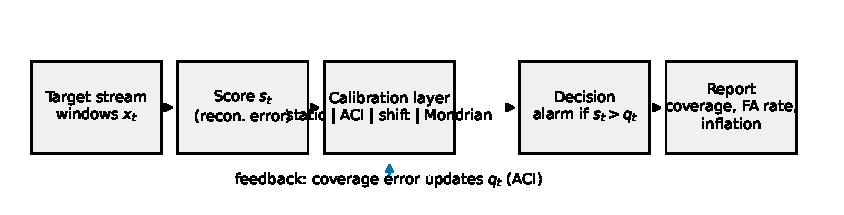
\includegraphics[width=\columnwidth]{fig_framework.pdf}
\caption{Calibration framework. A score producer (plain reconstruction encoder, frozen) feeds a calibration layer that estimates or tracks a threshold: static source quantile, online ACI with coverage feedback, divergence-shifted, or conditional (Mondrian). Deployments are summarized by normal-window coverage, alarm rate, false alarms, detection delay, and interval inflation.}
\label{fig:framework}
\end{figure}
